\chapter{I sensori inerziali negli Smartphone}
\label{cap:i_sensori_inerziali_negli_smartphone}

\section{Sensori presenti negli smartphone}
Dal lancio sul mercato del primo modello di IPhone nel 2007 gli smartphone hanno visto un enorme esplosione in popolarità tanto che al giorno d'oggi la maggior parte delle persone ne possiede almeno uno, che sia per uso personale o lavorativo.

Per offrire agli utenti un numero sempre crescente di funzionalità questi device fanno largo uso di sensori, montandone di tipi più disparati. I sensori più comuni sono {\bfseries l'accelerometro}, il {\bfseries giroscopio} e il gps, che consentono al device di sapere in ogni momento la sua posizione e il suo orientamento e vengono usati per i sistemi di tracking e per la rotazione automatica dello schermo; altri sensori molto diffusi negli smartphone sono: il sensore di prossimità, utilizzato per spegnere lo schermo quando l'utente avvicina il telefono all'orecchio durante una chiamata, il sensore di luminosità, che aggiusta la luminosità dello schermo in base alle condizioni di luce presenti e il lettore di impronte digitali, sempre più popolare, sta prendendo il posto delle comuni password per sbloccare il dispositivo o per convalidare le transazioni online (come i pagamenti elettronici).

Alcuni produttori di smartphone si spingono oltre, integrando sensori specifici per il monitoraggio dello stato di salute come: il termometro, il cardiofrequenzimetro, il sensore di umidità, e il pedometro (per misurare con esattezza il numero di passi compiuti dall'utente).

\begin{figure}[!htb]
    \centering
    \begin{subfigure}{0.4\textwidth}
        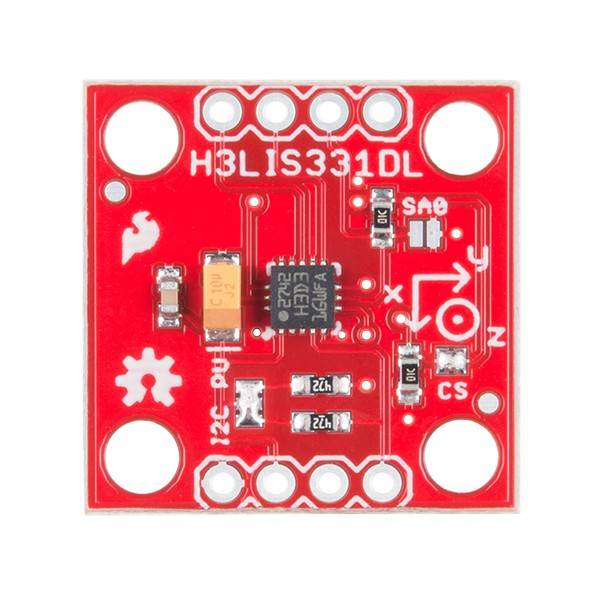
\includegraphics[width=\textwidth]{figures/accelerometer.jpg}
        \caption{Accelerometro (H3LIS331DL)}
        \label{fig:accelerometer}
    \end{subfigure}
    \begin{subfigure}{0.4\textwidth}
        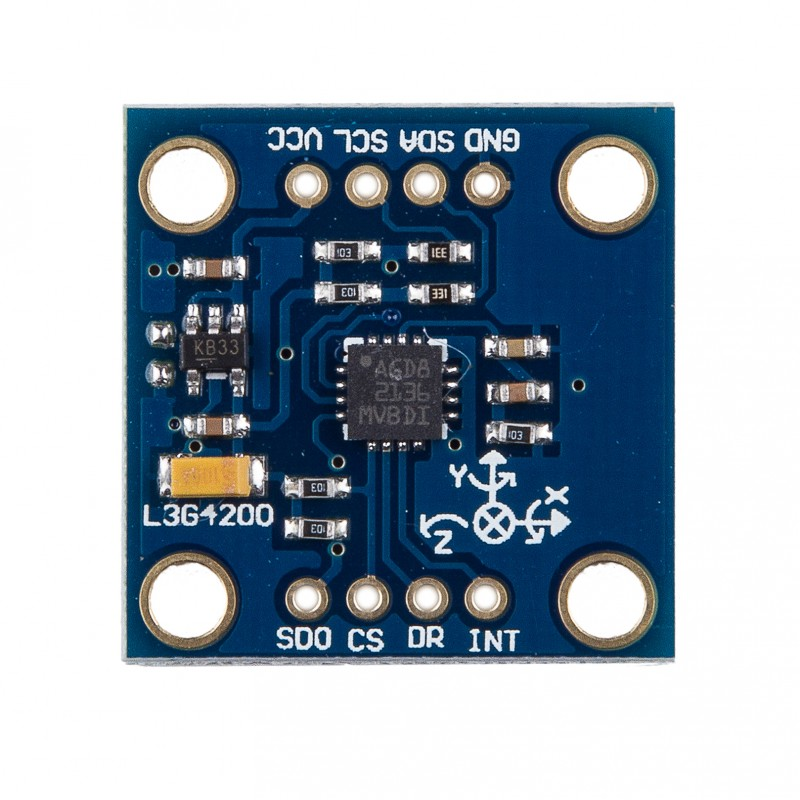
\includegraphics[width=\textwidth]{figures/gyroscope.jpg}
        \caption{Giroscopio (L3G4200D)}
        \label{fig:gyroscope}
    \end{subfigure}
    \caption{Esempio di due sensori MEMS integrati in un microchip}
    \label{fig:accelerometer_gyroscope}
\end{figure}

\section{L'accelerometro}
L'accelerometro (Figura \ref{fig:accelerometer}) è un dispositivo in grado di misurare l'accelerazione propria di un oggetto; concettualmente un accelerometro si comporta come una massa smorzata collegata ad una molla, quando il sensore risente di un'accelerazione la massa si sposta per inerzia comprimendola. Nei dispositivi commerciali spesso sono usati sensori con componenti capacitive o piezoelettriche in grado di convertire il moto della massa in un segnale elettrico comprensibile dagli strumenti di misura.

Negli ultimi anni l'uso dell'accelerometro è aumentato notevolmente a causa della sua diffusione in ambito civile, per questo con il moltiplicarsi delle applicazioni si è visto lo sviluppo di nuove tipologie di sensore, in grado di compiere misurazioni nella maniera più disparata; molti sensori lavorano in piano, ovvero sono progettati per essere sensibili solo su due assi cartesiani, per questo per creare un sensore triassale (sensibile a tutti e tre gli assi) si combinano due sensori uno perpendicolare all'altro.

Gli accelerometri più moderni spesso sono di tipo MEMS (Micro Electro-Mechanical Systems) prodotti con la stessa tecnologia utilizzata per creare i chip per questo hanno dimensioni veramente ridotte che gli consentono di integrare sullo stesso chip sia le componenti meccaniche di misurazione che quelle elettroniche di controllo. Il sensore MEMS è costituito da due condensatori dove la massa di prova è una delle due armature, quando l'accelerazione esterna sposta la massa la capacità dei condensatori varia ed è misurando questa variazione che è possibile quantificarla.

\section{Il Giroscopio}
Il giroscopio (Figura \ref{fig:gyroscope}) è un dispositivo fisico rotante inventato nel 1852 dal fisico Jean Bernard Léon Foucault; esso è costituito da un disco circolare montato su un sistema che lascia l'asse di rotazione libera di muoversi. Quando il disco è in rotazione l'orientamento del suo asse rimane parallelo e si oppone ad ogni tentativo di cambiamento in accordo con la legge di conservazione del momento angolare.

Oltre a quello meccanico esistono altri tipi di giroscopio, il giroscopio laser è composto da specchi e tubi cavi che direzionano un raggio laser in un percorso circolare e opera grazie al principio di Sagnac, il giroscopio a fibra ottica, invece, utilizza sottili fibre ottiche, mentre il giroscopio quantistico sfrutta fenomeni della meccanica quantistica per misurare l'asse di rotazione di un superconduttore; giroscopi di questo tipo sono molto precisi e stabili.

Al giorno d'oggi i giroscopi hanno svariati utilizzi dai sistemi di guida automatici per aerei, missili e sottomarini alle stedicam utilizzate per stabilizzare le macchine da presa nei film ai sistemi di guida inerziale dei satelliti.

L'effetto giroscopico è presente come effetto collaterale in tutti i dispositivi in rapida rotazione come i volani e gli hard disk per computer e deve essere tenuto in considerazione durante la progettazione.

I giroscopi MEMS, come gli accelerometri, sono dispositivi on-chip attualmente molto comuni nei dispositivi elettronici per il grande pubblico. Il primo a popolarizzare il giroscopio nell'elettronica di consumo fu Steve Jobs con il suo primo IPhone e da allora quasi ogni smartphone e tablet ne hanno integrato uno. Poiché il giroscopio permette il calcolo dell'orientamento e della rotazione spesso vengono combinati con accelerometri per riconoscere con maggior precisione i movimenti nello spazio 3D; proprio per questo sono molto diffusi anche nel mondo del gaming, integrati nei controller delle console (Dual-Shock di PlayStation, Joy-Con di Nintendo Switch) e nei sistemi di realtà virtuale (Oculus Rift, HTC Vive).